\chapter{Introduction} \label{chap:intro}

\section*{}

This chapter presents the context and motivation of this thesis, describing the main goals, it’s objectives and the expected results of work.

\section{Context and Motivation} \label{sec:context}

Nowadays current markets are changing, we can see more often the globalization phenomenon and with that organizations are compelled to streamline their business in order to achieve a favorable market position and be able to maintain or increase their competitiveness.

In our everyday lives software takes an important role, he is everywhere and is needed more often. When he is in development it is important to make it more efficiently and with more quality. For organizations that have software currently in development failures and errors are not allowed and each one of them implies increased costs and resources being wasted. To avoid this scenario and to achieve maximum efficiency and agility, their processes and their methodologies need to be less time consuming and more effortless so good practices need to be followed in order to allow them focus on what really matters: value creation. This will provide them advantages and make them more trustful.

Organizations need to ensure that their products and services consistently meet customer’s requirements, and that quality is consistently improved and certifications are a formal recognition of those ideals. Sadly those recognitions take too much time and effort and time being in some cases very painful and expensive.

SCAMPI is the Standard CMMI Appraisal Method for Process Improvement, the evaluation method of CMMI model. CMMI is a model for organizations to improve their processes and is required by many U.S. Government contracts, especially in software development. SCRAIM is the tool that is going to provide us the background and the base to work and simplify those kind of evaluations in order to save time and money. That way companies will deliver their products and services better, faster, and cheaper. 

\section{Goals and expected results} \label{sec:goals}

The main goal is of this dissertation is to develop a group of methodologies, techniques and tools integrated in the SCRAIM interface, that will make evaluations and certain parts of certifications easier and less painful for the SCRAIM users.
Although there are a number of life cycle and project management tools, few combine this with process management techniques. SCRAIM combines the two and will provide the users new features that will semi-automate the assessment for certification of an organization. 

\begin{figure}[h]
	\begin{center}
		\leavevmode
		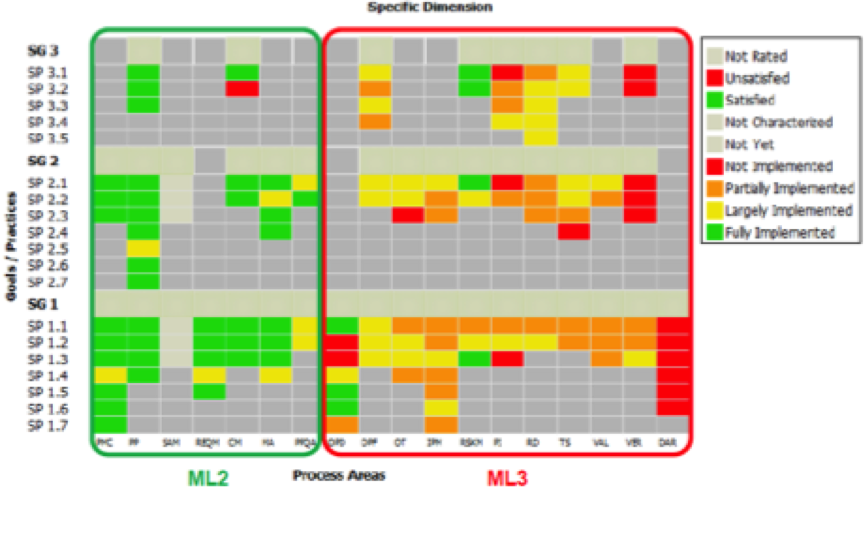
\includegraphics[width=0.86\textwidth]{thesis_goals}
		\caption{SCAMPI results}
		\label{fig:arch}
	\end{center}
\end{figure}

This image shows a matrix that is expected to have as output, and what is intended to do is:
\begin{itemize}
	\item Having SCRAIM as the basis for project activity take a sample of projects;
	\item Analyze the project activity in SCRAIM;
	\item Map the information of the produced articles to CMMI;
	\begin{itemize}
		\item Determine what are the good practices presented in SCRAIM, that can be mapped to CMMI;
		\item For each one of them investigate and conclude if that practice is being followed and fully satisfied;
	\end{itemize}
	\item Generate an matrix like the previous picture:
	\begin{itemize}
		\item Each column represents a good practice that needs to be followed and be satisfied;
	\end{itemize}
\end{itemize}	

The full-automated process is not yet feasible, so human intervention is still mandatory. With the use of SCRAIM, good practices will be followed and in the end the generated information will facilitate the decision making process. We can see many advantages of this innovation, and we believe that the application of this innovation will help reducing the costs and time of one evaluation using the SCAMPI method.

\section{Document structure} \label{sec:Structure}